\subsection{Digits and numbers 数字与数}
\begin{paracol}{2}
Digits are the building blocks of numbers.
\switchcolumn
数都是由数字所组成的。
\end{paracol}
\begin{figure}[!hbtp]
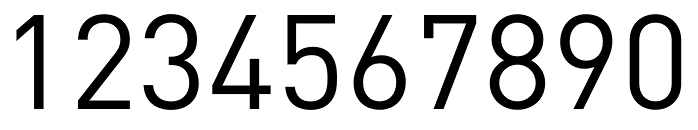
\includegraphics[width=0.8\textwidth]{digits.png}
\caption{Digits 数字\label{fig:digit}}
\end{figure}
\begin{paracol}{2}
The position of each digit in a number tells what the digit means. For example, 2143 can be expaned as $2000+100+40+3$.
\switchcolumn
数字在数的不同的位置代表了不同的意义。例如 2143 可以表示为 $2000+100+40+3$.
\end{paracol}
\begin{table}[htp]
\centering
\begin{tabular}{|p{.8cm}<{\centering}|p{.8cm}<{\centering}|p{.8cm}<{\centering}|p{.8cm}<{\centering}|p{.8cm}<{\centering}|p{.8cm}<{\centering}|p{.8cm}<{\centering}|p{.8cm}<{\centering}|p{.8cm}<{\centering}|p{.8cm}<{\centering}|p{.8cm}<{\centering}|p{.8cm}<{\centering}|}
\toprule	
\multicolumn{3}{|c|}{billions period}& \multicolumn{3}{|c|}{millions period} & \multicolumn{3}{|c|}{thousands period} & \multicolumn{3}{|c|}{ones period}\\ \hline
\rotatebox[origin=c]{90}{\parbox[c]{2cm}{\centering \begin{spacing}{0.8}hundred-billions\end{spacing}}}&\rotatebox[origin=c]{90}{\parbox[c]{2cm}{\centering \begin{spacing}{0.8}ten-billions\end{spacing}}}& \rotatebox[origin=c]{90}{\parbox[c]{2cm}{\centering billions}}&
\rotatebox[origin=c]{90}{\parbox[c]{2cm}{\centering \begin{spacing}{0.8}hundred-millions\end{spacing}}}&\parbox[t]{2mm}{ \rotatebox[origin=c]{90}{ten\\-millions}}& \parbox[t]{2mm}{\rotatebox[origin=c]{90}{millions} }&
\rotatebox[origin=c]{90}{\parbox[c]{2cm}{\centering \begin{spacing}{0.8}hundred-thousands\end{spacing}}}&\rotatebox[origin=c]{90}{\parbox[c]{2cm}{\centering \begin{spacing}{0.8}ten-thousands\end{spacing}}}& \parbox[t]{2mm}{\rotatebox[origin=c]{90}{thousands} }&
\parbox[t]{2mm}{\rotatebox[origin=c]{90}{hundred}}&\parbox[t]{2mm}{ \rotatebox[origin=c]{90}{ten}}& \parbox[t]{2mm}{\rotatebox[origin=c]{90}{ones} }\\
\midrule
&&7&5&5&0&2&6&2&1&0&1\\
\bottomrule
\end{tabular}
\caption{World population (by July 1st, 2017) 世界人口(截止至2017年7月1日)\\
7 billion, 755 million, 262 thousand, 101. 75亿5026万2101\label{tab:numbers}}
\end{table}

\begin{example}
Tell what each number means. 解释每个数\\
\begin{tabular}{cccc}
a. 4,823& b. 8,910 & c. 219,181,193 & d. 4,200,000,000
\end{tabular}
\end{example}

\begin{example}
Given the standard form 写出每个表示代表的数\\
\begin{tabular}{ll}
a. 4000+300+20+1 & b. 8000+5 \\
c. nine hundred six billion, three million & d. 27 million, 321 thousands, 456
\end{tabular}
\end{example}
\newpage
